%!TEX ROOT=main.tex
\chapter{Software}
Tato kapitola se zaměří na popis vývojového prostředí, používaného programovacího jazyka a knihoven.
\begin{figure}[H]
    \label{fig:sw_diagram}
    \caption{Digram připojených periférii k MCU}
    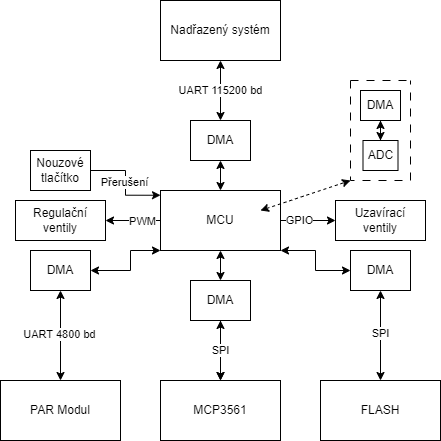
\includegraphics[width=0.9\textwidth]{pictures/sw_diagram.png}
\end{figure}
\section{Vývojové prostředky}
MCU STM32F407ZG6 je postaveno na architektůře Arm Cortex M4 s přidaným jádrem a instrukcemi pro výpočty plouvoucích čísel.
Programování MCU probíha v programovacím prostředí od ST Microeletronics STM32CubeIDE, které má v sobě zabudovaný kompilátor, prostředí pro debugging a a prostředky pro nahrání SW do MCU.
\begin{figure}[H]
    \caption{Ukázka vývojového prostředí STM32CubeIDE pro mikroprocesory STM32}
    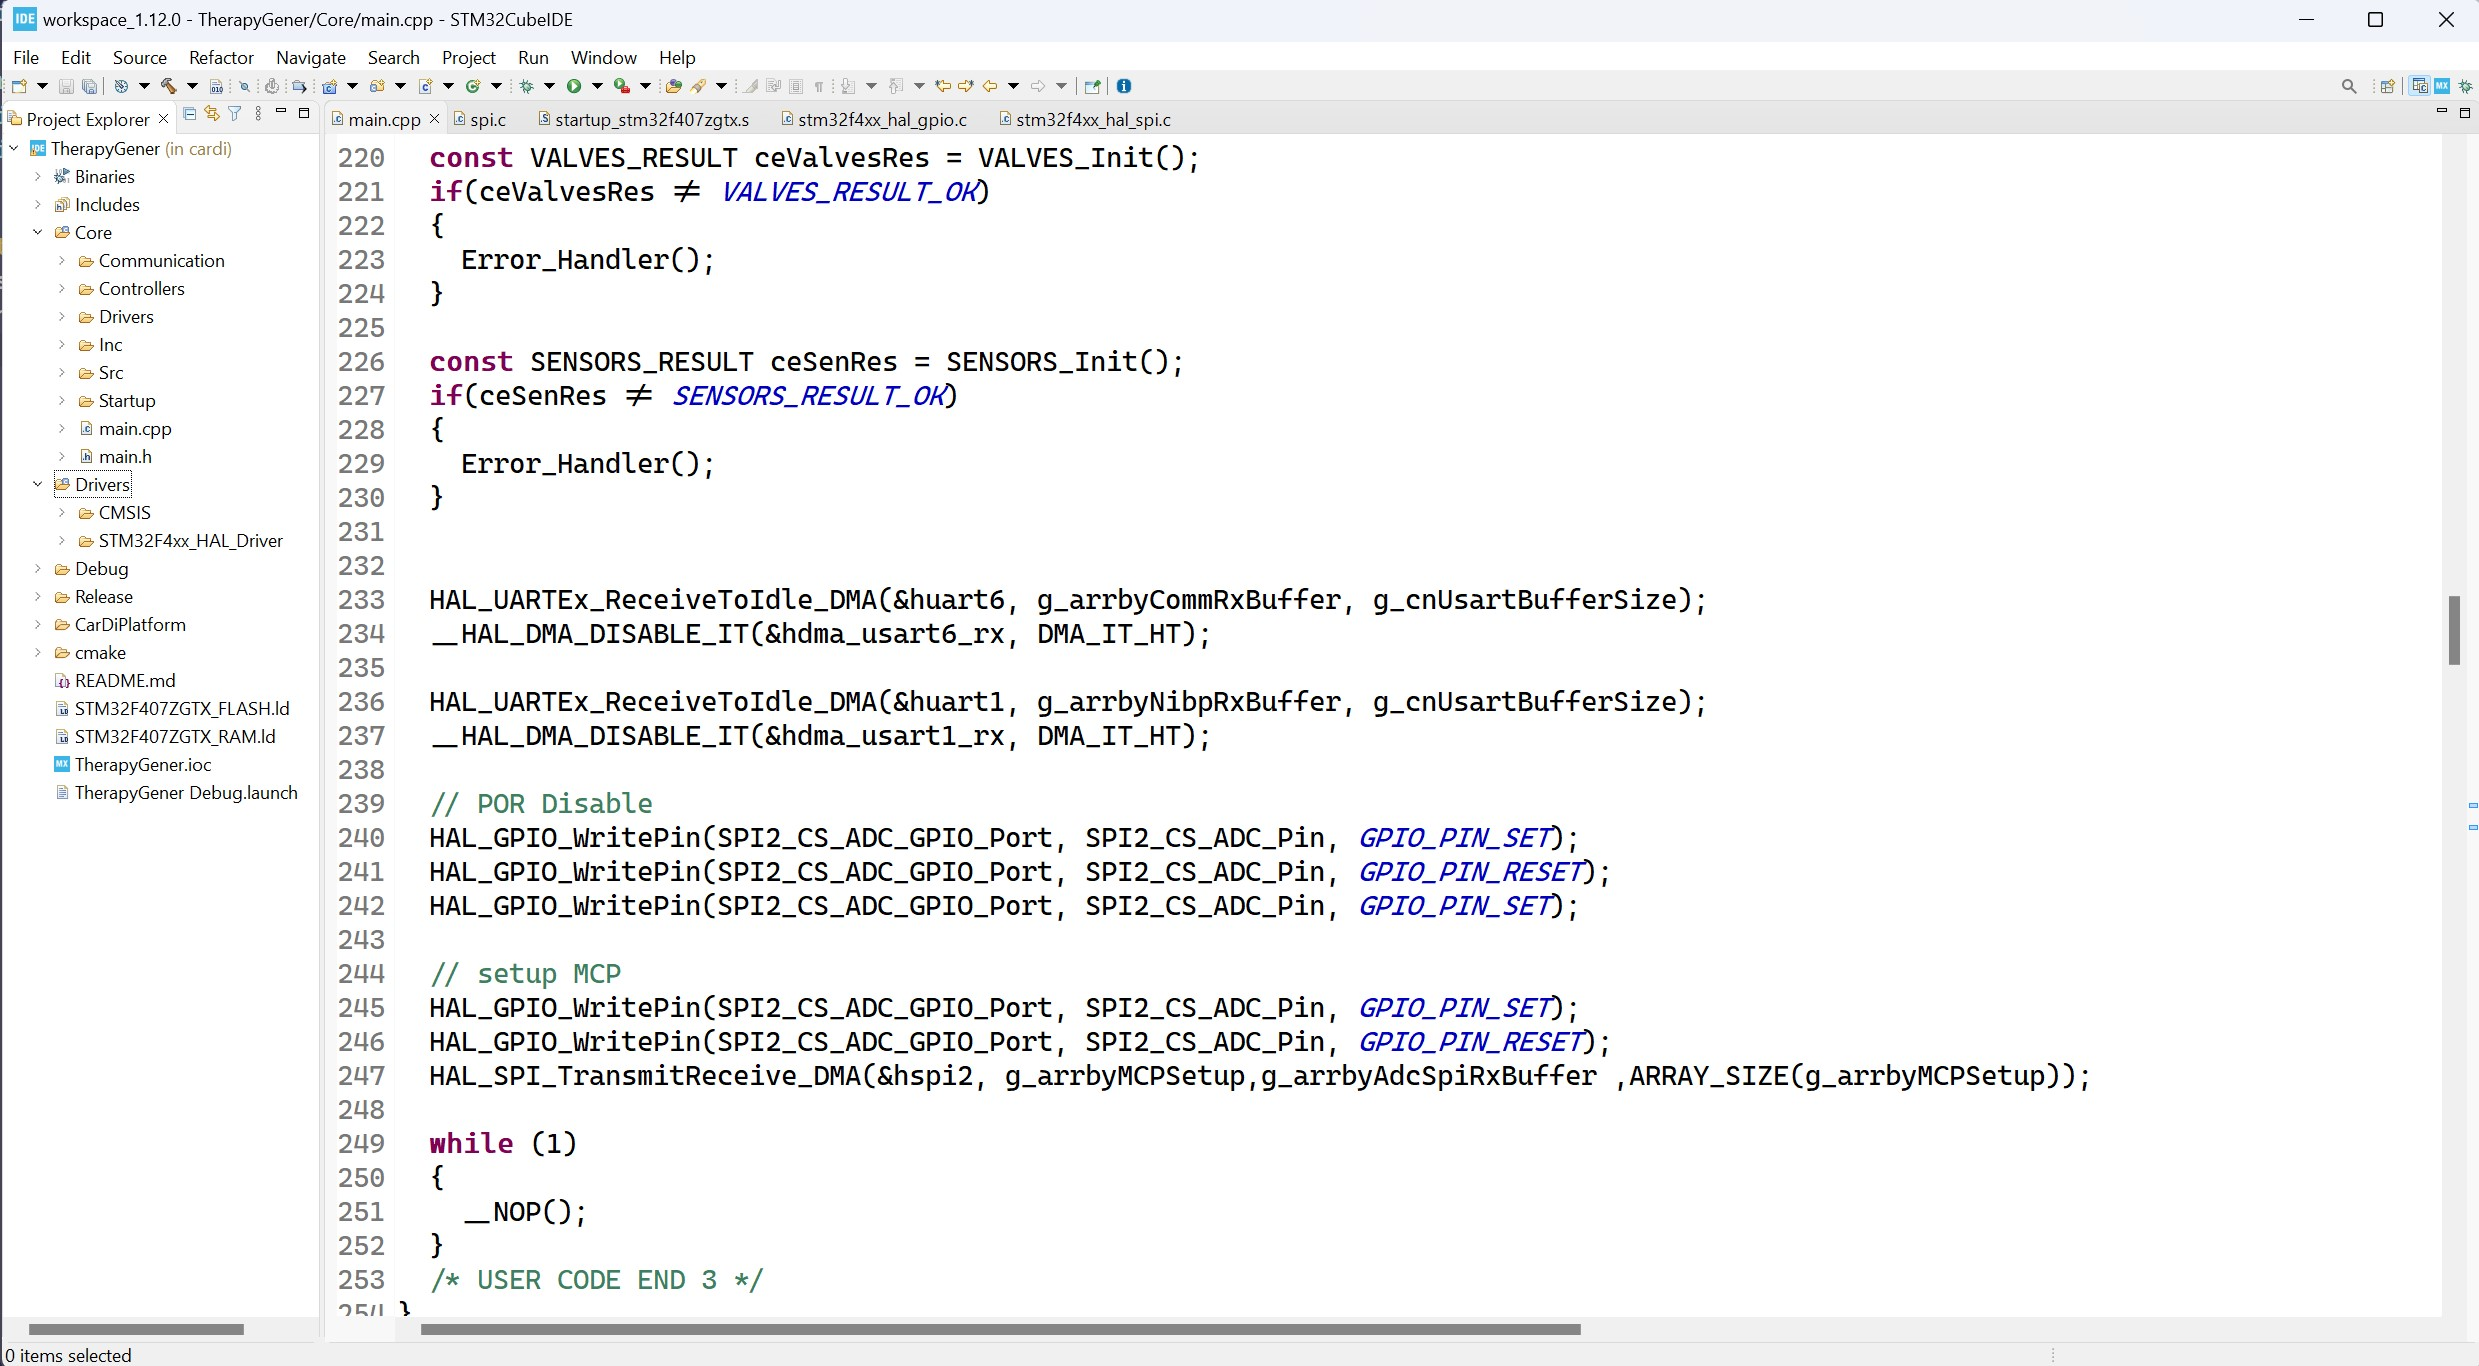
\includegraphics[width=0.9\textwidth]{pictures/cubeide.jpg}
\end{figure}
STM32CubeIDE také sprostředkovává ovladače pro komunikaci s internímy periferiemy a prostředí pro konfiguraci MCU.
\begin{figure}[H]
    \caption{Konfigurace GPIO pinů MCU}
    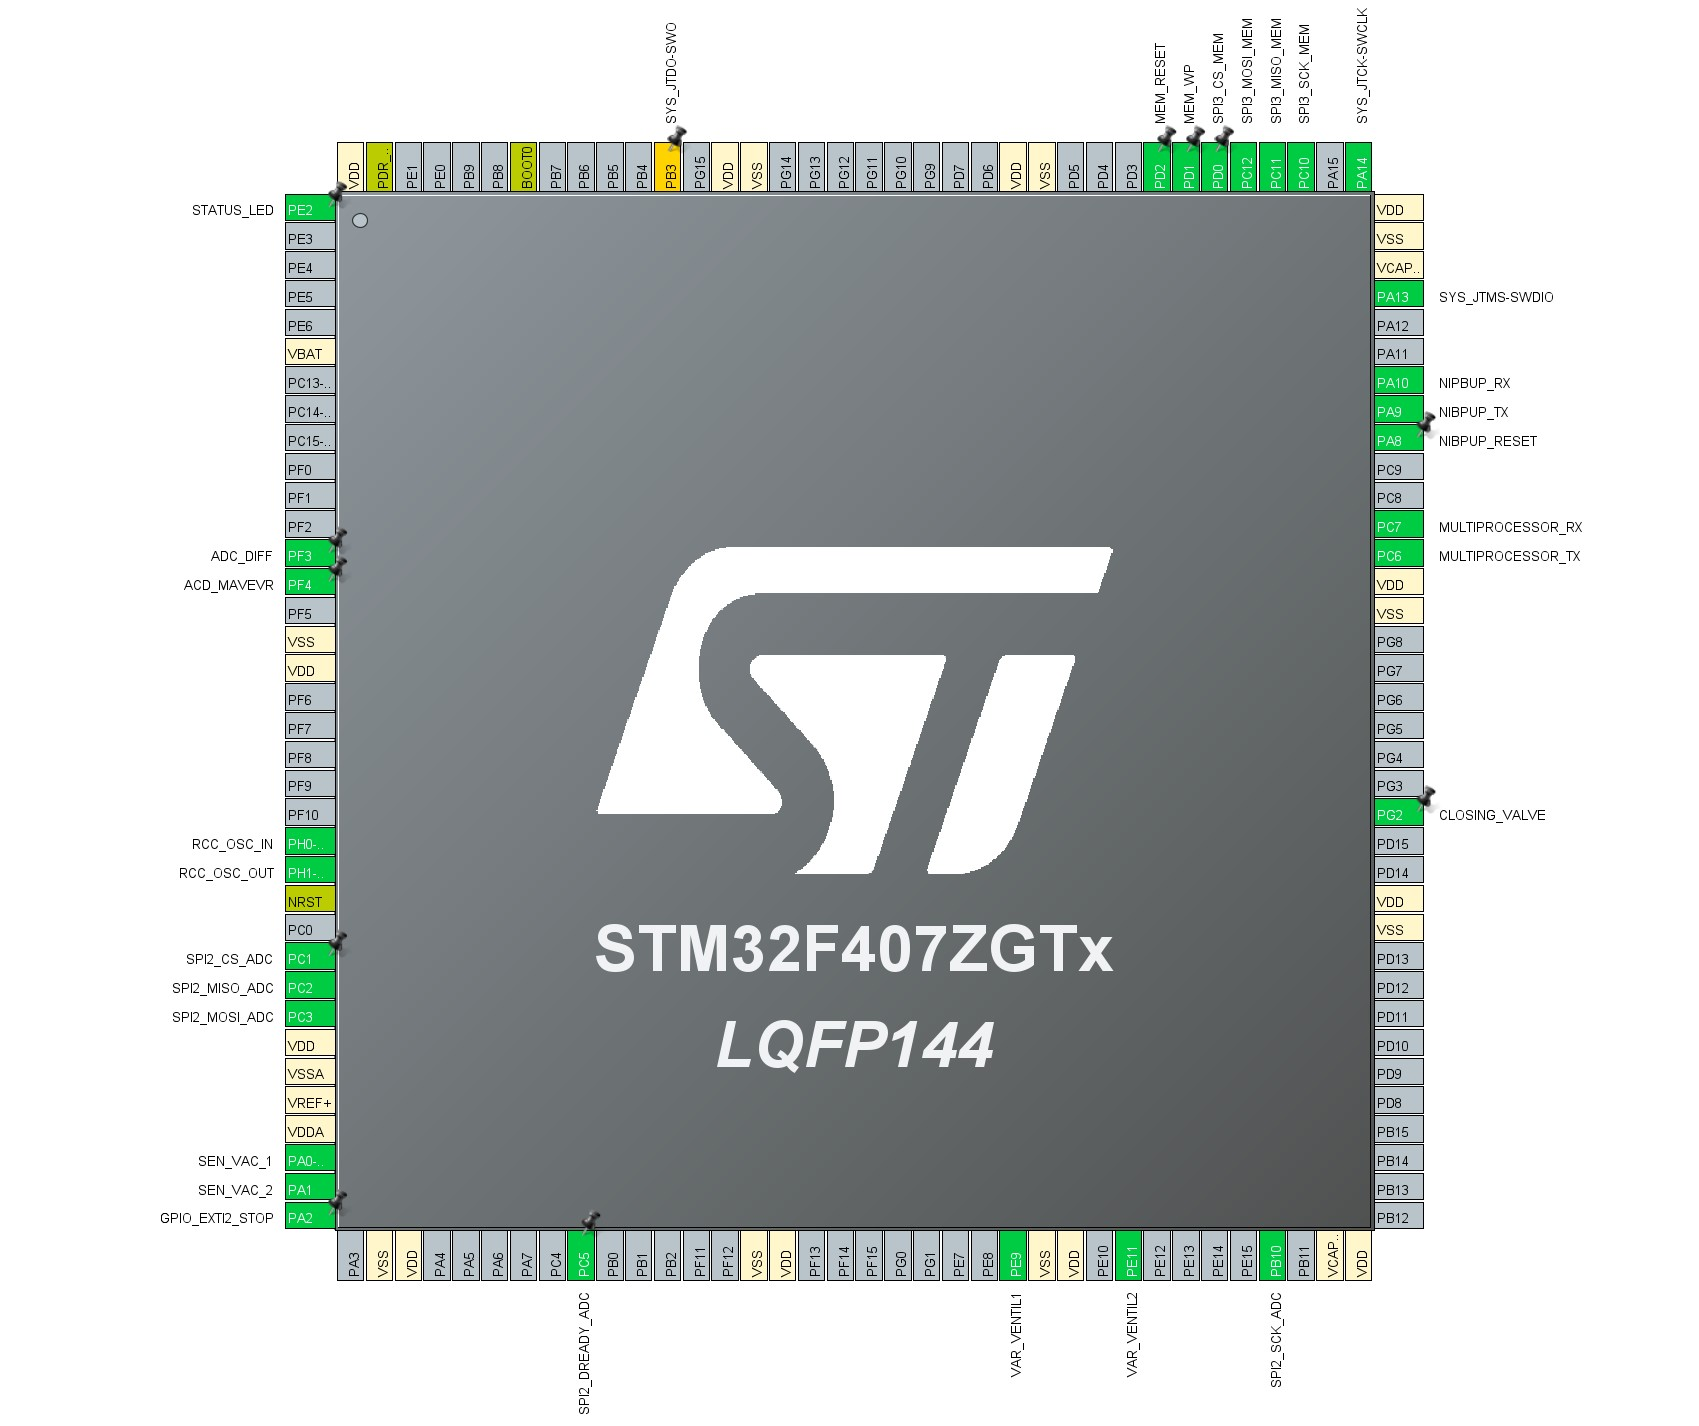
\includegraphics[width=0.9\textwidth]{pictures/mcu_settings.jpg}
\end{figure}
Po zvolení konfigurace MCU, STM32CubeIDE vygeneruje základní softwarovou inicializaci periférií.
\par
Nahrání SW a debuggování MCU musí být provedeno přes programátor od firmy ST Microeletronics ST-LINK.
\begin{figure}[H]
    \caption{Programátor ST-LINK V2/ISOL}
    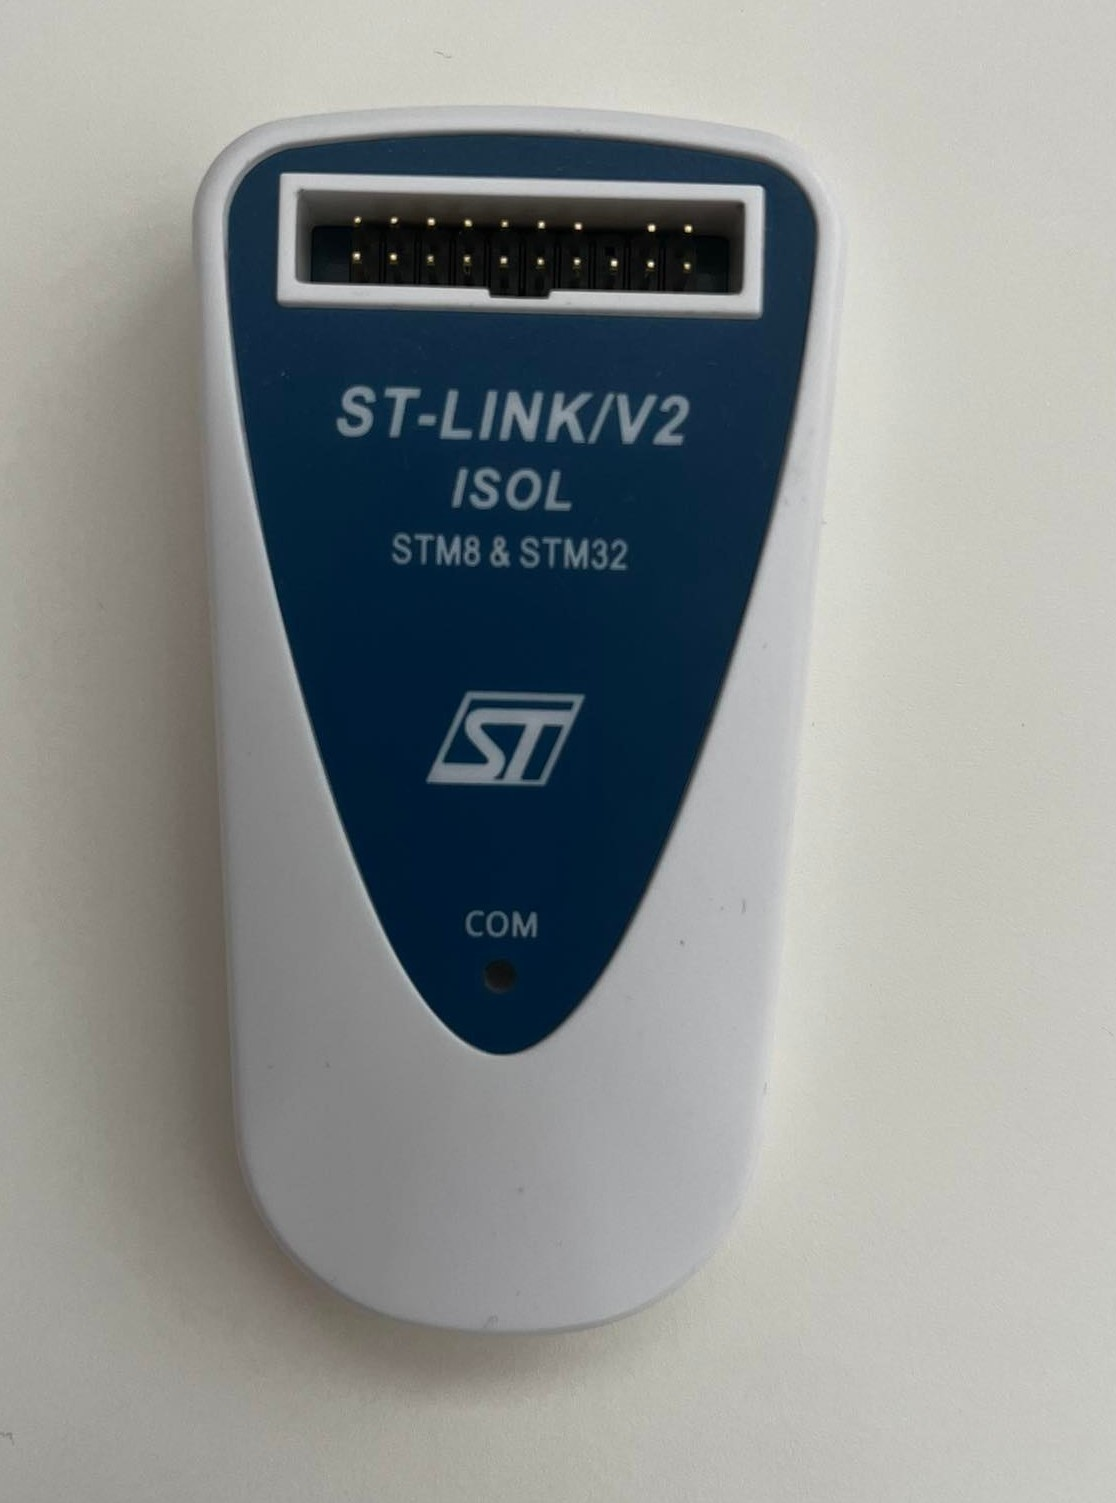
\includegraphics[width=0.5\textwidth]{pictures/stlink.jpg}
\end{figure}
MCU využívá komunikační protokol Serial Wire Debug vyvinutý přímo firmou ST M. Pro připojení k DPS je použitý speciální kabel od firmy TagConnect TCP2030, který se připojí na kontakt na povrchu DPS.
\begin{figure}[H]
    \caption{Programovací kabel TagConnect TCP2030}
    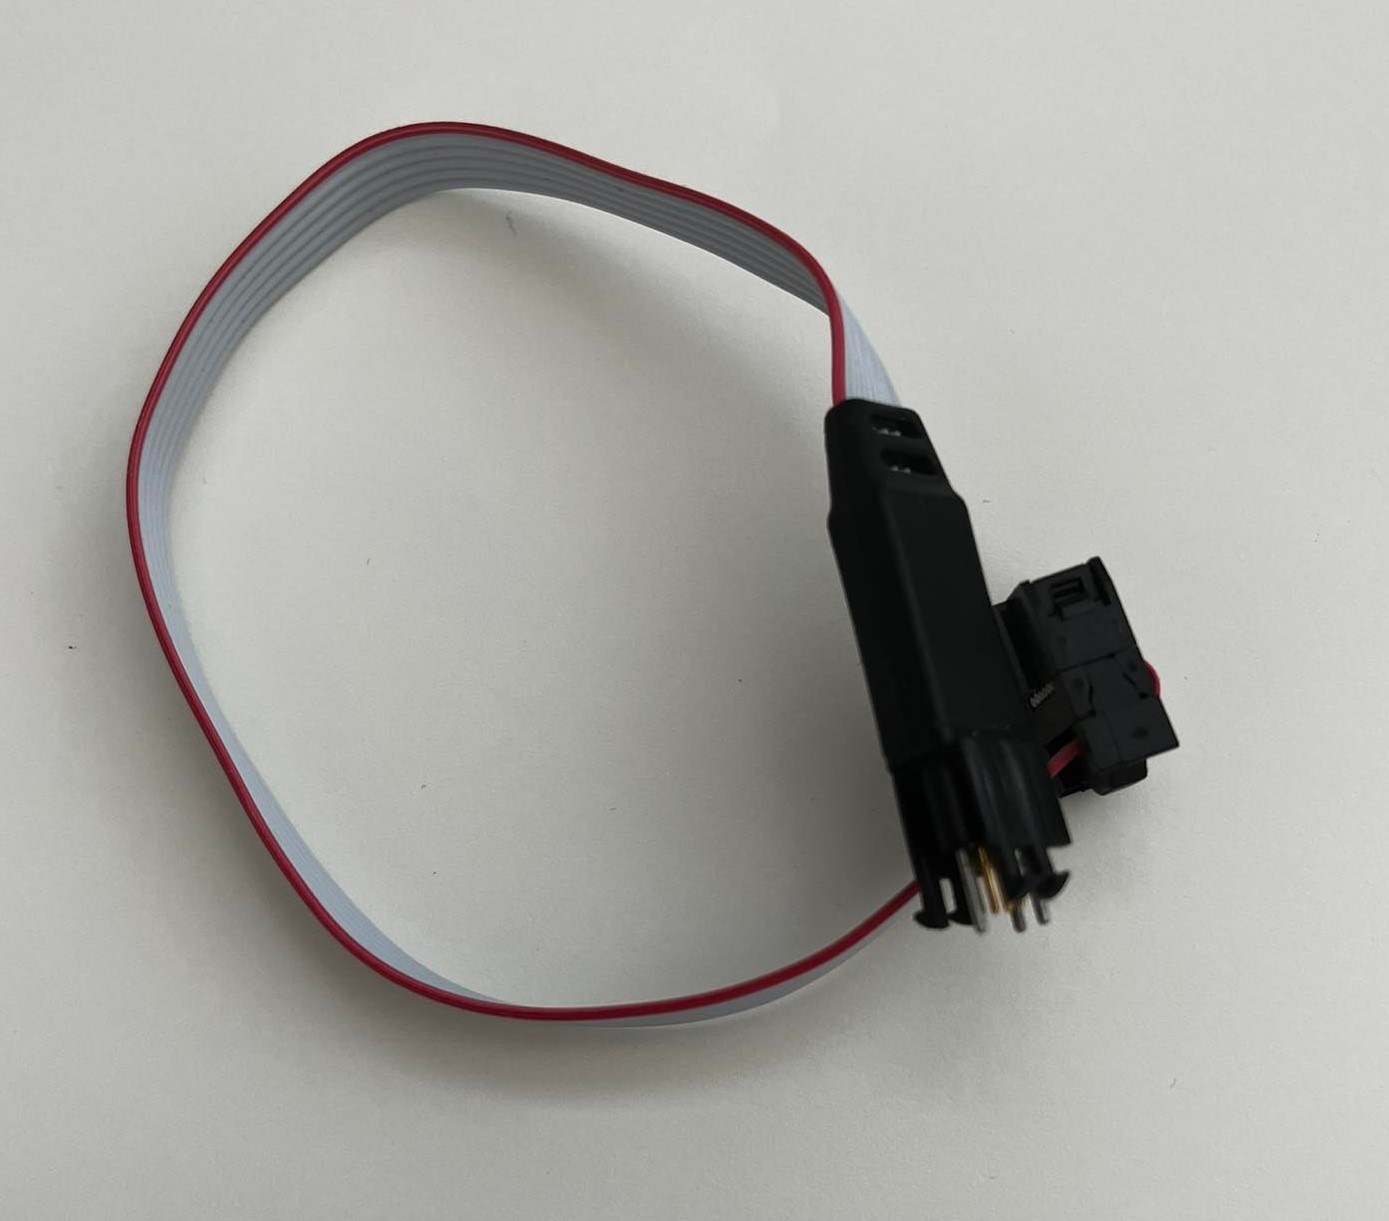
\includegraphics[width=0.6\textwidth]{pictures/tcp2030.jpg}
\end{figure}
\section{Komunikace s nadřazeným systémem}
Nadřazený systém je systém, se kterým interaktuje uživatel a zároveň sprostředkovává příkazy pro ovládání DPS a případný sběr naměřených dat z DPS.
Nadřazený systém také slouží jako bezpečnostní bariéra, omezením přístupu uživatele k "žívým" potenciálně nebezpečným částím přístroje a to z hlediska hardware i vymezením příkazů na ovládání DPS.
\par
Komunikace probíhá pomocí asynchroního seriového rozhraní UART s přenosovou rychlostí 115200 baud.
UART umožňuje zasílaní jakýkoliv dat čí provedení úkonů ze strany DPS, záleží na definici příkazů. Definice příkazů musí být z stejná ze strany DPS i nadřazeného systému.
Přenosová rychlost byla 115200 baud zvolena pro optimální rychlost přenosu dat, ale i pro spolehlivý přenos.
Jelikož UART je asynchroní komunikace, záleží na přesném časování příchozích a odchozích dat,
jinak hrozí korupce dat a nevalidní přenos a případné nesplnění příkazů.